%% The first command in your LaTeX source must be the \documentclass command.
%%
%% Options:
%% twocolumn : Two column layout. Do not use twocolumn for papers submitted to CEUR-WS!
%% hf: enable header and footer.
\documentclass[
% twocolumn,
% hf,
]{ceurart}

%%
%% One can fix some overfulls
\sloppy

%%
%% Minted listings support 
%% Need pygment <http://pygments.org/> <http://pypi.python.org/pypi/Pygments>
\usepackage{listings}
\usepackage{xcolor}
\usepackage{booktabs}
\usepackage{amsfonts}
\usepackage{amssymb}
\usepackage{amsmath}
\usepackage{tipa} % IPA phonetic symbols (\textipa)
%% auto break lines
\lstset{breaklines=true}

\usepackage[macros]{argumentation}
\usepackage{_macros}

\hyphenation{Tweety-Pro-ject}

%\newcommand{\todo}[1]{\textcolor{magenta}{TODO: #1}}
\newcommand{\agon}{\textsc{AgonProject}\xspace}
\newcommand{\tweety}{\textsc{TweetyProject}\xspace}

%%
%% end of the preamble, start of the body of the document source.
\begin{document}

%%
%% Rights management information.
%% CC-BY is default license.
\copyrightyear{2026}
\copyrightclause{Copyright for this paper by its authors.
  Use permitted under Creative Commons License Attribution 4.0
  International (CC BY 4.0).}

%%
%% This command is for the conference information
\conference{The Sixth International Workshop on Systems and Algorithms for Formal Argumentation,
  September 14, 2026, Barcelona, Spain}

%%
%% The "title" command
\title{AgonProject: An Online Platform for Exploring Approaches to Formal Argumentation}

%%
%% The "author" command and its associated commands are used to define
%% the authors and their affiliations.
\author[]{Lars Bengel}[%
email=lars.bengel@fernuni-hagen.de,
]
\cormark[1]

\author[]{Matti Berthold}[%
email=matti.berthold@fernuni-hagen.de,
]

\author[]{Oleksandr Dzhychko}[%
email=oleksandr@dzhychko.de,
]

\address[]{Artificial Intelligence Group, University of Hagen, Germany}

\author[]{Matthias Thimm}[%
email=matthias.thimm@fernuni-hagen.de,
]

%% Footnotes
\cortext[1]{Corresponding author.}

%%
%% The abstract is a short summary of the work to be presented in the
%% article.
\begin{abstract}
Formal Argumentation provides a rigorous foundation for modelling and evaluating reasoning in the presence of conflicting information. However, students and newcomers often find its zoo of formalisms challenging to understand due to their diverse semantics, underlying algorithms, and implementation details. This paper presents \agon, a web-based interface that provides unified access to \tweety, a comprehensive collection of Java libraries for logical aspects of artificial intelligence and knowledge representation. The platform enables users to construct argumentation instances, execute different reasoning tasks, and compare the behaviour of multiple formalisms through an intuitive, interactive interface. By abstracting away installation and programming requirements, the system lowers the barrier to experimentation while preserving access to state-of-the-art implementations. \agon is designed as a learning tool that encourages exploration, visualisation, and comparative analysis, allowing users to develop a deeper understanding of the similarities and differences between argumentation formalisms and their associated semantics. The platform is suitable for classroom demonstrations, hands-on exercises, and self-directed learning, making formal argumentation more accessible to students and practitioners alike.
\end{abstract}

%%
%% Keywords. The author(s) should pick words that accurately describe
%% the work being presented. Separate the keywords with commas.
%\begin{keywords}
  
%\end{keywords}

%%
%% This command processes the author and affiliation and title
%% information and builds the first part of the formatted document.
\maketitle

\section{Introduction}

\emph{Formal argumentation} is a major research area in the field of \emph{knowledge representation and reasoning}.
In his seminal paper in 1995, Dung~\cite{DBLP:journals/ai/Dung95} introduced the \emph{abstract argumentation framework (AF)}, which still remains the foundational model of formal argumentation until today.
In essence, AFs represent argumentation scenarios as directed graphs, where the nodes are abstract arguments, and the edges are disagreements (or attacks) between them. 
However, in the thirty years since the introduction of abstract argumentation frameworks, the literature has seen a wide range of works that propose different extensions of AFs~\cite{DBLP:books/hofa/BaroniGT17,DBLP:books/hofa/GabbayGST21,DBLP:books/hofa/GabbayKST24}.
These extensions range from introducing additional relations between arguments~\cite{DBLP:conf/ecsqaru/CayrolL05a,DBLP:conf/argmas/NielsenP06,DBLP:journals/ai/Modgil09,CaminadaKRU25} to introducing weights~\cite{DBLP:journals/flap/Bistarelli021} or probabilities~\cite{DBLP:books/hofa/HunterPPRT21} and many other aspects~\cite{DBLP:books/hofa/GabbayGST21,DBLP:books/hofa/GabbayKST24}.

The large number of formal extensions of argumentation frameworks is accompanied by an equally diverse collection of implementations. These range from highly specialised contenders of the \emph{International Competition on Computational Models of Argumentation (ICCMA)}\footnote{\url{https://argumentationcompetition.org}}, to visual interfaces, e.\,g. \textsc{PyArg}~\cite{DBLP:conf/ai3/OdekerkenBB23} and \textsc{AFx-ray}~\cite{DBLP:conf/icail/Xia0BL25}. The work of Persiani et al.~\cite{DBLP:conf/comma/PersianiGBKK24} gives an excellent overview of the landscape of these tools and implementations. Amongst them, \tweety~\cite{DBLP:conf/kr/Thimm14, DBLP:journals/ki/Thimm17a} probably offers the most comprehensive library of implementations of and around formal argumentation. Yet \tweety only offers text based web-interfaces for a select few tasks: Inconsistency Measurement, Defeasible Logic Programming, and Assumption-based Argumentation.

The goal of the current paper is hence to provide a unified \emph{visual} web-interface to the argumentation libraries of \tweety, such that users have a platform that gives an easily accessible overview of the field,
introduces the basics and capabilities of the different formalisms, and
can be used by experts to support research and paper writing.

In particular, \agon supports the following functionalities for several major argumentation formalisms:
\begin{itemize}
    \item Framework construction and visualisation via an interactive graph editor,
    \item Semantical evaluation of argumentation frameworks,
    \item Exporting frameworks in several formats, including \LaTeX,
    \item Random generation of argumentation frameworks,
    \item Tutorials and formal definitions, as well as references to the literature.
\end{itemize}

Section~\ref{sec:general} gives a more detailed overview over the features of \agon. Section~\ref{sec:modules} details the modules handling the different argumentation formalisms. Finally, Section~\ref{sec:outlook} offers an outlook on future features and some concluding remarks.
% \todo{paragraph on existing tools and how important applications and visualisation are}
% \begin{itemize}
%     \item \tweety~\cite{DBLP:conf/kr/Thimm14, DBLP:journals/ki/Thimm17a}, \textsc{PyArg}~\cite{DBLP:conf/ai3/OdekerkenBB23}, \textsc{AFx-ray}~\cite{DBLP:conf/icail/Xia0BL25}, \emph{International Competition on Computational Models of Argumentation (ICCMA)}\footnote{\url{https://argumentationcompetition.org}}, etc.
%     \item The work of Persiani et al.~\cite{DBLP:conf/comma/PersianiGBKK24} gives an excellent overview of the landscape of tools and implementation for formal argumentation.
% \end{itemize}

% \todo{paragraph on our main goal}
% The argumentation literature offers a wide variety of different formalisms, each with different advantages and capabilities.
% It is therefore crucial for any practitioner to be able to \todo{continue: get an overview of suitable approaches? }
% \begin{itemize}
%     \item gives an easily accessible overview of the field,
%     \item introduces the basics and capabilities of the different formalisms
%     \item can be used to support research and paper writing
% \end{itemize}

\section{General Overview}\label{sec:general}
%\todo{maybe a bit more detail regarding the overall ambition; briefly describe what falls under formal argumentation}
\agon (from Greek \textit{ag\=on}, meaning a \enquote{contest} or \enquote{struggle}) provides an interactive, graph-based editor for exploring different approaches to formal argumentation directly in the browser.
The platform is available under

\begin{center}
    \url{http://agon.tweetyproject.org}%\url{https://agonproject.aig.fernuni-hagen.de/}%\url{https://agonproject.tweetyproject.org}
\end{center}

At the moment, \agon already supports a broad range of different approaches to formal argumentation, see also \autoref{fig:mainview} for an overview:

\begin{enumerate}
    \item \textit{abstract argumentation frameworks (AFs)}~\cite{DBLP:journals/ai/Dung95},
    \item \textit{bipolar argumentation frameworks (BAFs)}~\cite{DBLP:journals/ijar/CayrolL13,DBLP:journals/ker/CohenGGS14}, 
    \item \textit{abstract dialectical frameworks (ADFs)}~\cite{DBLP:conf/kr/BrewkaW10,DBLP:conf/ijcai/BrewkaSEWW13},
    \item \textit{incomplete argumentation frameworks (iAFs)}~\cite{DBLP:journals/ai/Coste-MarquisDKLM07,DBLP:journals/ai/BaumeisterJNNR21},
    \item \textit{probabilistic argumentation frameworks (PAFs)}~\cite{DBLP:conf/tafa/LiON11,DBLP:books/hofa/HunterPPRT21},
    \item \textit{argumentation frameworks with collective attacks (SetAFs)}~\cite{DBLP:conf/argmas/NielsenP06,DBLP:journals/flap/BikakisCDFP21}.
\end{enumerate}

A detailed overview over the functionalities for each approach is given below and in \autoref{sec:modules}.

\begin{figure}[ht]
    \centering
    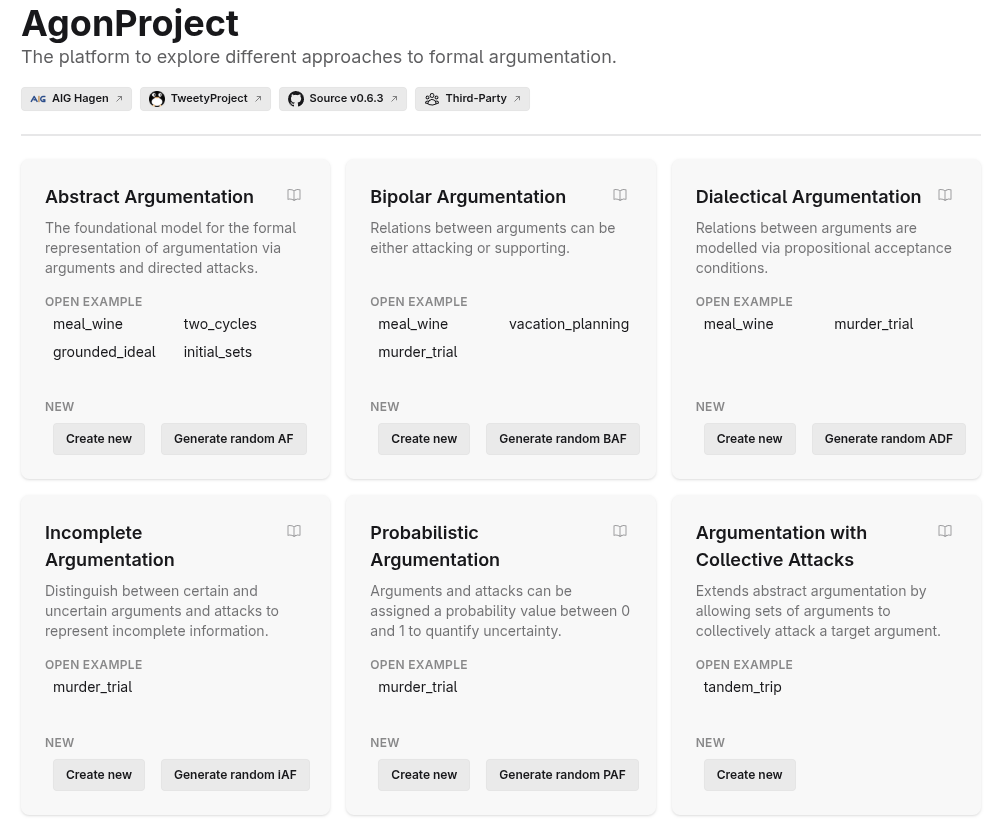
\includegraphics[width=0.65\linewidth]{figures/main.png}
    \caption{Landing page of \agon with overview of included argumentation formalisms.}
    \label{fig:mainview}
\end{figure}

\agon is a client-side single-page application built with Vue 3 and TypeScript, bundled with Vite.
The UI is styled using Tailwind CSS v4 with the DaisyUI component library. 
Interactive graph visualisation is handled by the \texttt{aig-graph-component}\footnote{\url{https://github.com/aig-hagen/aig_graph_component}}, a public library for interactive graph visualisation.
Computational reasoning tasks are delegated to a backend REST API that wraps \tweety~\cite{DBLP:conf/kr/Thimm14,DBLP:journals/ki/Thimm17a}, which provides implementations of all relevant argumentation formalisms, reasoning tasks and semantics.
Importantly, \agon is in general decoupled from any specific backend implementation and can be readily extended to interface with alternative backends.
\agon is released under the GNU general public license 3.0 and the source code is openly available under

\begin{center}
    \url{https://github.com/aig-hagen/AgonProject}
\end{center}


The central goal of \agon is to provide a comprehensive overview of the field of formal argumentation and the available approaches for modelling argumentation.
To facilitate that, the following features are available for all formalisms.

\paragraph{Framework Construction and Visualisation}
Users can easily construct and manipulate argumentation frameworks directly via an interactive graph editor.
Argument positioning can be adjusted manually or with the help of several automated layout algorithms, for instance, directed, circular, radial, and force-directed approaches, implemented via \texttt{Graphviz}~\cite{DBLP:journals/spe/GansnerN00}.
The graph editor also includes a physics-based simulation for organic graph arrangement.

\paragraph{Semantical Reasoning}
Semantic evaluation is performed by delegating queries to the \tweety backend.
There is a wide variety of argumentation semantics available for all approaches, for a detailed list see below.
For all extension-based semantics, the evaluation supports three well-known computational tasks: enumerating all extensions as well as enumerating the credulously (resp. sceptically) acceptable arguments~\cite{DBLP:books/hofa/DvorakD17}.
Individual extensions can also be highlighted directly in the argumentation framework, utilising the corresponding labeling-based representation~\cite{DBLP:journals/sLogica/CaminadaG09}.
The user can also open multiple evaluation windows at the same time to easily compare results of different semantics.

\paragraph{Export and Sharing}
All argumentation frameworks can be exported to \LaTeX{}, utilising the \texttt{argumentation}\footnote{\url{https://ctan.org/pkg/argumentation}} \LaTeX{}-package.
The \texttt{argumentation} package provides high-level syntax for creating argumentation frameworks via TikZ, including attack, support as well as collective relations and comes with easily configurable visual styles.
An optional grid-overlay in the graph editor can be used to facilitate consistent node placement in the \LaTeX{} output.
Furthermore, the argumentation frameworks can also be saved as an SVG or exported to standard exchange formats such as the AF-Format of ICCMA and the Trivial Graph Format (TGF).
Argumentation frameworks can easily be shared with others via a generated share-URL.

\paragraph{Random Generation}
\agon provides random argumentation framework generators backed by configurable graph generation algorithms from the \texttt{networkX}\footnote{\url{https://networkx.org/}} Python package.
In total, there are eight graph generation algorithms supported, including the Erdös-Renyi, Watts-Strogatz or Barabasi-Albert approaches.
In addition to the algorithm-specific parameters the \agon-interface also provides parameters for specific argumentation framework related parameters.

\paragraph{Tutorials and References}
\agon comes with more than ten step-by-step tutorials that guide the user through framework construction, semantical evaluation and other advanced interactions with the tool.
Beyond that, \agon includes an extensive glossary of definitions for all relevant concepts and semantics, each with references to the corresponding publications.
For each argumentation formalism, a selection of example argumentation frameworks is provided to illustrate the capabilities of each formalism.


\section{Module Overview}\label{sec:modules}
In the following, we give an overview of all six argumentation modules.
For that, we briefly recall the basic definitions and specifics of each formalism, list the supported semantics and describe module-specific features.

\subsection{Abstract Argumentation Frameworks}

Abstract argumentation frameworks as introduced by~\citeauthor{DBLP:journals/ai/Dung95}~(\citeyear{DBLP:journals/ai/Dung95}) form the foundation of formal argumentation. They represent argumentation scenarios as directed graph, where arguments are nodes and conflicts (attacks) between them are edges.

\begin{definition}\label{def:af}
    An \emph{abstract argumentation framework} (\AF) is a tuple $(\arguments,\attacks)$, where $\arguments$ is a finite set of arguments and $\attacks$ is an attack relation $\attacks\subseteq \arguments\times\arguments$.
\end{definition}

AFs are evaluated under different semantics, each yielding a set of extensions (sets of arguments) representing valid combinations of accepted arguments. An argument is credulously accepted if it appears in at least one extension and sceptically accepted if it appears in all extensions.
Beyond the classical semantics of Dung~\cite{DBLP:journals/ai/Dung95}, the argumentation literature offers a large collection of different extension-based semantics.
All extension-based semantics currently supported by \agon are listed in \autoref{tab:ext-semantics}.

\begin{table}[ht]
    \renewcommand{\arraystretch}{1.2}
    \centering
    \caption{Overview of available semantics for AFs, BAFs, iAFs, PAFs and SetAFs in \agon.}
    \begin{tabular}{@{}p{0.28\linewidth}p{0.68\linewidth}@{}}
            \toprule
            \textbf{Group} & \textbf{Semantics}\\
            \midrule
            Classical semantics & Conflict-free, admissible, complete, grounded, preferred, stable~\cite{DBLP:journals/ai/Dung95}\\
            Admissibility-based semantics& Ideal~\cite{DBLP:journals/ai/DungMT07}, semi-stable~\cite{verheij1996two,DBLP:conf/comma/Caminada06}, eager~\cite{caminada2007comparing}, strong admissibility~\cite{DBLP:conf/comma/Caminada14}, initial sets~\cite{DBLP:journals/jancl/XuC18}, unchallenged~\cite{DBLP:conf/comma/BengelT22}\\
            Non-admissible semantics & Naive~\cite{DBLP:journals/ai/BaroniG07}, CF2~\cite{DBLP:journals/ai/BaroniGG05a}, SCF2~\cite{DBLP:conf/ki/CramerT19}, stage~\cite{verheij1996two}, stage2~\cite{DBLP:journals/logcom/DvorakG16}, (strongly) undisputed sets~\cite{DBLP:conf/aaai/Thimm23}\\
            Weak-admissibility-based semantics & w-admissible, w-complete, w-grounded, w-preferred~\cite{DBLP:conf/aaai/BaumannBU20}\\
            \bottomrule
        \end{tabular}
    \label{tab:ext-semantics}
\end{table}

In addition to the extension-based semantics, \agon also supports a variety of \emph{argument-ranking semantics}, which define a total ordering on a frameworks arguments according to some measure of acceptability~\cite{DBLP:conf/aaai/BonzonDKM16}.
The following well-known argument-ranking semantics are currently included in \agon: Burden-based~\cite{DBLP:conf/sum/AmgoudB13a}, Categoriser~\cite{DBLP:conf/ksem/PuLZL14}, Counting~\cite{DBLP:conf/cogsci/PuLZL15}, Discussion-based~\cite{DBLP:conf/sum/AmgoudB13a}, Iterated Graded Defense~\cite{DBLP:conf/ijcai/GrossiM15}, Serialisability-based~\cite{DBLP:conf/comma/BlumelT22}, Social Argumentation~\cite{DBLP:conf/ijcai/LeiteM11}, Strategy-based~\cite{DBLP:conf/jelia/MattT08} and Tuples~\cite{DBLP:journals/jair/CayrolL05}.

Moreover, \agon also supports \emph{serialisability}~\cite{DBLP:journals/argcom/Thimm22,DBLP:conf/comma/BengelT22}.
Serialisability describes an iterative construction scheme of admissibility-based extensions yielding a series of initial sets~\cite{DBLP:journals/jancl/XuC18} of the respective reducts~\cite{DBLP:conf/aaai/BaumannBU20} -- called a \emph{serialisation sequence} -- that represents the order of construction of admissible sets.
\agon provides the ability to enumerate the serialisation sequences for various selection and termination criteria~\cite{DBLP:journals/argcom/Thimm22}.
In addition to that, it also has an interactive mode, where the user can assemble a serialisation sequence by resolving the argumentation framework step-by-step.

\autoref{fig:aa} shows an \AF in \agon and its evaluation based on extension- and ranking-based semantics, with the categoriser argument-ranking highlighted directly in the AF.

\begin{figure}[ht]
    \centering
    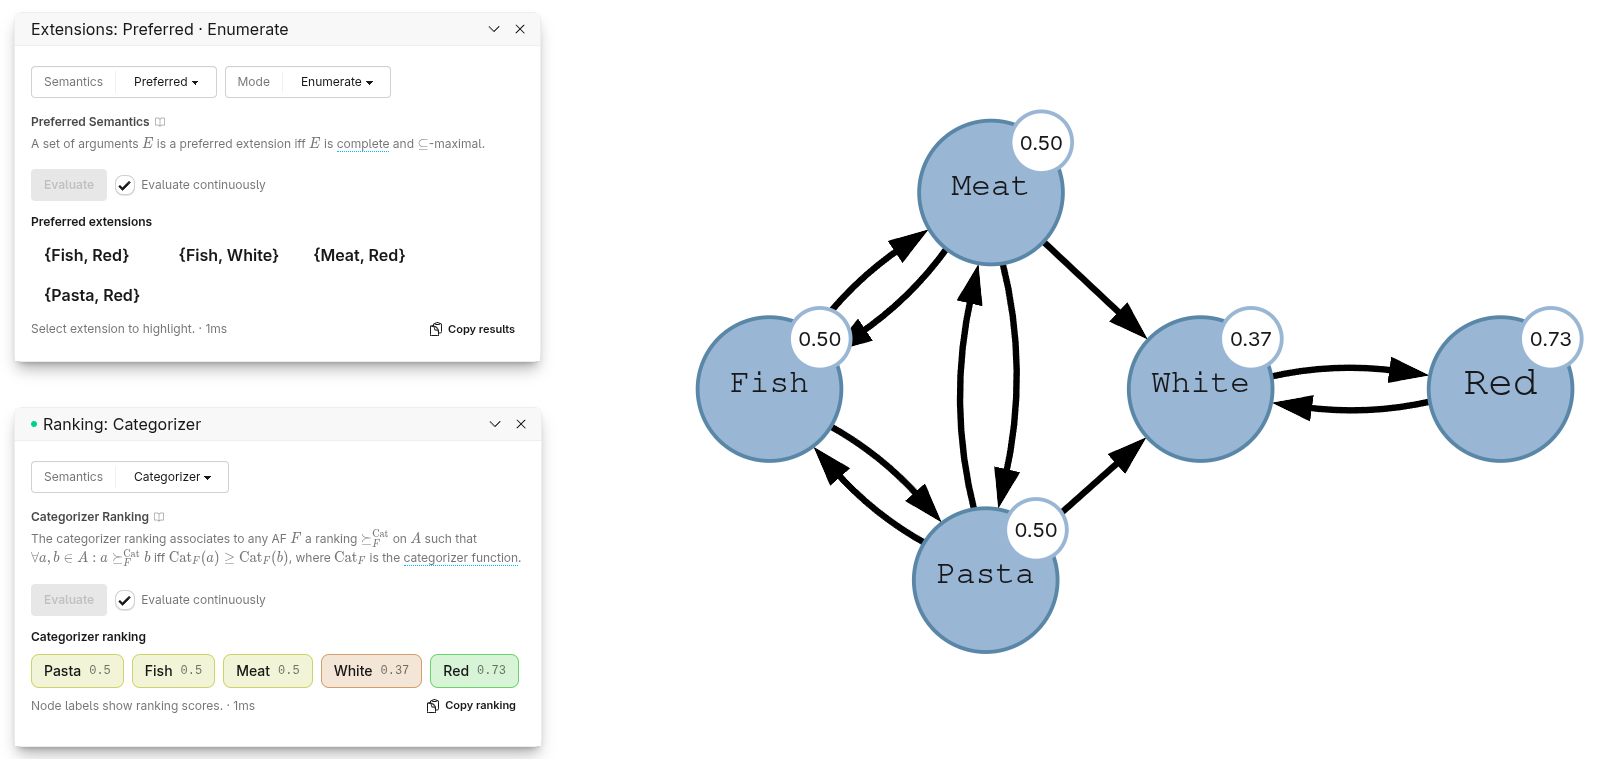
\includegraphics[width=0.9\linewidth]{figures/aa.png}
    \caption{An exemplary abstract argumentation framework and its semantical evaluation via the preferred semantics and the categoriser ranking-semantics in \agon. The Categoriser values of each argument are directly annotated in the \AF.}
    \label{fig:aa}
\end{figure}

\subsection{Bipolar Argumentation Frameworks}

Bipolar argumentation frameworks~\cite{DBLP:conf/ecsqaru/CayrolL05a,CaminadaKRU25} extend AFs with a binary support relation between arguments. 

\begin{definition}\label{def:baf}
    A \emph{bipolar argumentation framework} (\BAF) is a tuple $(\arguments,\attacks, \supports)$, where $\arguments$ is a finite set of arguments, $\attacks\subseteq \arguments\times\arguments$ is the attack relation and $\supports\subseteq \arguments\times\arguments$ is the support relation.
\end{definition}

There are several different ways how the support relation can be interpreted in a \BAF~\cite{DBLP:journals/ijar/CayrolL13,DBLP:journals/ker/CohenGGS14}, ultimately leading to different interpretations of the extension-based semantics.
One approach are the \emph{coalition-based semantics}~\cite{DBLP:journals/ijis/CayrolL10}, which consider coalitions of arguments, \ie, $\subseteq$-maximal, conflict-free sets that are connected via the support relation $\supports$.
These coalitions are then considered as arguments in an \AF, with attacks between them depending on whether they contain arguments that attack each other, such that the \sem-extensions of the coalition-\AF then induce \sem-extensions of the original \BAF.
Alternatively, one can distinguish between the \emph{deductive support}~\cite{DBLP:conf/comma/BoellaGTV10} ($a$ supporting $b$ means the acceptance of $a$ implies the acceptance of $b$) and the \emph{necessary support}~\cite{DBLP:conf/ictai/NouiouaR10} ($a$ supporting $b$ means the acceptance of $a$ is necessary for the acceptance of $b$).
For all three approaches, all extension-based semantics from \autoref{tab:ext-semantics} are available in \agon.

\subsection{Abstract Dialectical Frameworks}

Abstract dialectical frameworks allow arguments to have arbitrary acceptance conditions; i.e., each node of the argumentation graph is associated with a classical propositional formula containing its parents as atoms~ \cite{DBLP:conf/kr/BrewkaW10,DBLP:conf/ijcai/BrewkaSEWW13}.

\begin{definition}\label{def:adf}
    An \emph{abstract dialectical framework} (\ADF) is a tuple $(\arguments,\links,\conditions)$ where $\arguments$ is a set of arguments, $\links \subseteq \arguments\times\arguments$ is a set of links and $\conditions$ is a set of propositional formulae $\{\phi_a\}_{a\in\arguments}$ over $\arguments$, called \emph{acceptance conditions}.%\footnote{In the original definition of ADFs \citep{DBLP:conf/ijcai/BrewkaSEWW13}, acceptance conditions are given as total functions $C_a : 2^{par(a)} \mapsto \{\tr, \f\}$ over the parents $par(a)$ of each $a$. In our work, we exclusively use the representation as propositional formulae for convenience. Note that both representations are functionally equivalent.}.
\end{definition}

In contrast to all other argumentation formalisms considered here, the semantics of ADFs are based on three-valued interpretations $\model : \arguments \mapsto \{\tr, \f, \un\}$, similar to the labeling-based approach for AFs.
Due to the higher expressiveness and computational complexity of ADFs compared to AFs~\cite{DBLP:journals/ai/StrassW15}, no reduction to AFs exists.
Therefore, only the three-valued versions of the classical semantics~\cite{DBLP:conf/kr/BrewkaW10,DBLP:conf/ijcai/BrewkaSEWW13}, cf. \autoref{tab:ext-semantics} and the naive semantics~\cite{DBLP:journals/ai/StrassW15} are available for ADFs in \agon.
To make the construction of ADFs, in particular the acceptance conditions, more accessible, \agon provides a graphical interface for setting up acceptance conditions and automatically infers the links between arguments from the given conditions.

\autoref{fig:adf} shows an \ADF in \agon with one of the stable models highlighted in the graph.

\begin{figure}[ht]
    \centering
    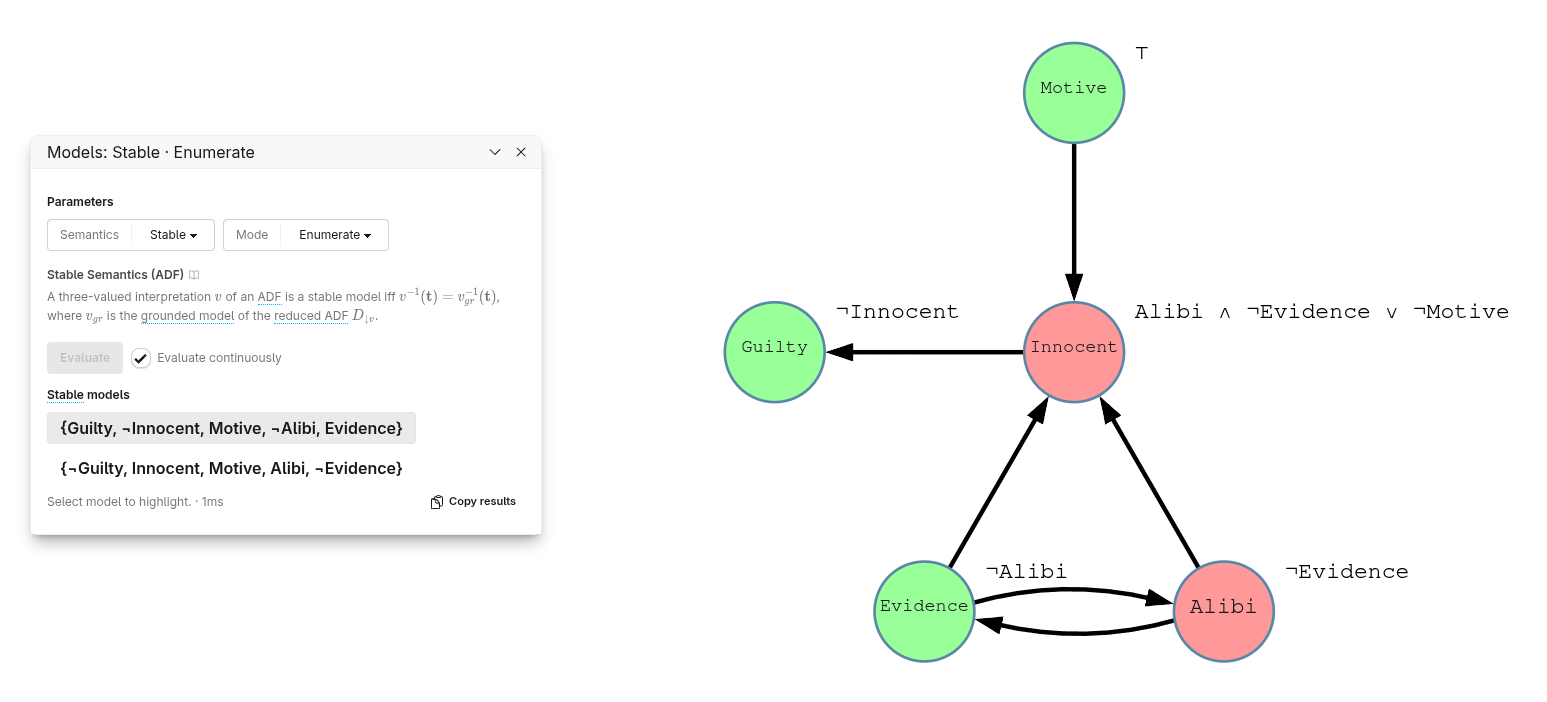
\includegraphics[width=0.9\linewidth]{figures/adf.png}
    \caption{Exemplary abstract dialectical framework in \agon and the evaluation window for enumerating stable models. The first stable model is highlighted in the graph.}
    \label{fig:adf}
\end{figure}

\subsection{Incomplete Argumentation Frameworks}

Incomplete argumentation frameworks~\cite{DBLP:journals/ai/Coste-MarquisDKLM07,DBLP:journals/ai/BaumeisterJNNR21} model uncertainty of both arguments and attacks.

\begin{definition}\label{def:iaf}
    An \emph{incomplete argumentation framework} (\iAF) is a tuple $(\arguments,\arguments^?,\attacks,\attacks^?)$, with $\arguments$ as the set of \emph{definite arguments}, $\arguments^?$ the set of \emph{uncertain arguments} as well as the set of \emph{conditionally definite attacks} $\attacks\subseteq (\arguments \cup \arguments^?)\times(\arguments \cup \arguments^?)$ and the set of \emph{uncertain attacks} $\attacks^?\subseteq (\arguments \cup \arguments^?)\times(\arguments \cup \arguments^?)$.
\end{definition}

A \emph{completion} of \iAF is any $\AF^* = (\arguments^*, \attacks^*)$ such that $\arguments \subseteq \arguments^* \subseteq \arguments \cup \arguments^?$ and $\attacks|_{\arguments^*} \subseteq \attacks^* \subseteq (\attacks \cup \attacks^?)|_{\arguments^*}$.
We then say that some $E\subseteq\arguments$ is a \emph{possible \sem-extension} of an $\iAF$, iff there exists some completion $\AF^*$ of $\iAF$ such that $E \in \sem(\AF^*)$.
On the other hand, if $E \in \sem(\AF^*)$ for all completions $\AF^*$ of $\iAF$, then $E$ is a \emph{necessary \sem-extension} of $\iAF$.
We can extend the same notion to credulous/sceptical acceptance.
\agon supports all extension-based semantics listed in \autoref{tab:ext-semantics} for iAFs under both possible and necessary reasoning for extension enumeration and credulous/sceptical reasoning.

\subsection{Probabilistic Argumentation Frameworks}

Probabilistic argumentation frameworks~\cite{DBLP:books/hofa/HunterPPRT21,DBLP:conf/tafa/LiON11} associate a probability to each argument and attack. Correspondingly, their semantics predict the likelihood with which a set of arguments can be accepted.

\begin{definition}\label{def:paf}
    A \emph{probabilistic argumentation framework} (\PAF) is a tuple $(\arguments, \attacks, \probdist)$, such that $\AF = (\arguments,\attacks)$ is an abstract argumentation framework and $\probdist : \arguments \cup \attacks \mapsto (0, 1]$ is a probability distribution over the elements of \AF.
\end{definition}

For the semantical evaluation of PAFs, we utilise the \emph{constellation-based approach} and consider credulous and sceptical acceptance of arguments, and no extension enumeration.
For the evaluation, we then take into account all viable constellations of arguments and attacks, \ie, all sub-frameworks with a probability $p > 0$.
The probability of credulous/sceptical acceptance \wrt the semantics \sem of an argument $a\in\arguments$ in the \PAF is defined as the sum of probabilities $p_{\AF_i}$ of the sub-frameworks $\AF_i$ in which the argument $a$ is credulously/sceptically accepted \wrt \sem.
For that, all extension-based semantics of \autoref{tab:ext-semantics} are supported.
Furthermore, \agon allows for the exact computation of probabilities as well as an approximate calculation based on a Monte-Carlo simulation~\cite{DBLP:conf/tafa/LiON11}.


\subsection{Argumentation Frameworks with Collective Attacks}

Argumentation frameworks with collective attacks, or \SetAF~\cite{DBLP:conf/argmas/NielsenP06,DBLP:journals/flap/BikakisCDFP21} broaden the attack notion to take into account that several arguments may be necessary to defeat another argument.

\begin{definition}\label{def:setaf}
    An \emph{argumentation framework with collective attacks} (\SetAF) is a tuple $(\arguments,\attacks)$, where $\arguments$ is a finite set of arguments and $\attacks$ is the attack relation $\attacks\subseteq 2^{\arguments}\times\arguments$.
\end{definition}

For the semantical evaluation of SetAFs, we utilise a polynomial-size reduction to AFs~\cite{DBLP:journals/logcom/ModgilB11}, which introduces several meta-arguments for each set-attack.
Due to that, all extension-based semantics from \autoref{tab:ext-semantics} are available for SetAFs.
In the graph-editor, the set-attacks are rendered dynamically as directed hyperedges, where the edges of the source arguments meet seamlessly at a junction point before reaching the target argument.
For a set-attack $(S, t) \in \attacks$, the coordinates of the junction point $j$ are computed as a weighted combination of the centroid $\bar{c} = \frac{1}{|S|}\sum_{a \in S} p_a$ and the target argument $t$ as $j = 0.25 \cdot \bar{c} + 0.75 \cdot p_t$, where $p_a$ is the position of argument $a$.
For a smooth curve of the set-attack, each attacker-to-junction segment is then rendered as a cubic Bézier curve $B(u)$, $u \in [0,1]$, with $B(0) = p_a$ and $B(1) = j$, whose control points are chosen such that $B'(1)$ is parallel to $j - p_t$, ensuring all source curves arrive at $j$ tangent to the junction-to-target direction.

\autoref{fig:setaf} shows an example \SetAF in \agon with the \LaTeX{}-export window.
The look of the generated TikZ-image can be adjusted via various style parameters.

\begin{figure}[ht]
    \centering
    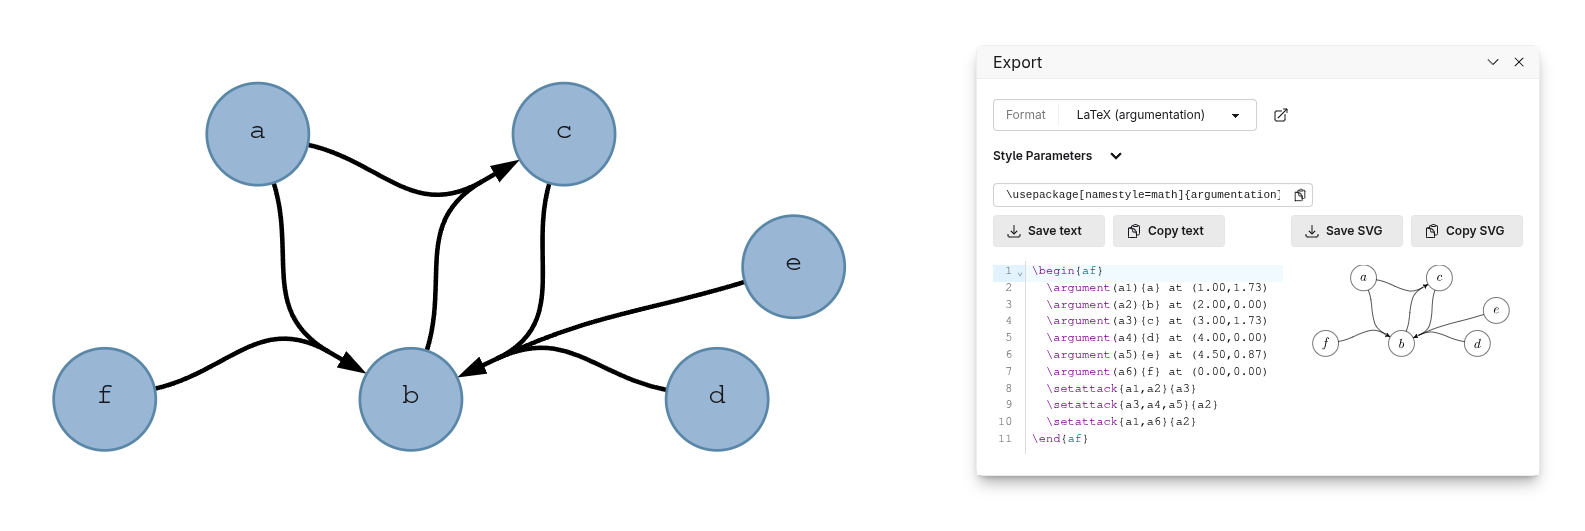
\includegraphics[width=0.9\linewidth]{figures/setaf.png}
    \caption{A \SetAF in \agon together with the export window, showing the auto-generated \LaTeX{}-code and SVG-preview.}
    \label{fig:setaf}
\end{figure}

\section{Outlook and Conclusion}\label{sec:outlook}

This paper presented \agon, a unified web-based interface for exploring formal argumentation through the implementations provided by \tweety. By combining interactive visualisation, framework construction, semantic evaluation, export utensils, and integrated tutorials, formal definitions, and references within a single platform, \agon lowers the barrier to working with a wide range of argumentation formalisms. Its primary goal is to make formal argumentation more accessible, enabling students, researchers, and practitioners to experiment with different models and semantics without requiring extensive programming expertise or complex software installation. Through interactive exploration and comparison of different formalisms, the platform supports classroom teaching and self-directed learning.

The current version of \agon already covers several major argumentation formalisms, but the platform is intended to evolve alongside the field. Planned extensions include support for additional formalisms such as Assumption-Based Argumentation (ABA)~\cite{DBLP:books/sp/09/DungKT09,DBLP:books/hofa/CyrasFST17}, Weighted Argumentation Frameworks~\cite{DBLP:journals/flap/Bistarelli021}, Bipolar Set-based Argumentation Frameworks (BSAFs)~\cite{DBLP:conf/kr/BertholdR024}, and claim-augmented argumentation frameworks~\cite{DBLP:conf/ecai/Rapberger20,DBLP:journals/ai/DvorakRW23}. We also plan to integrate benchmark generators from the ICCMA ecosystem~\cite{DBLP:journals/argcom/BistarelliKLLMRST25,DBLP:journals/ai/JarvisaloLN25} and additional reasoning tasks, including explanation-based approaches that help users understand why particular arguments are accepted or rejected.

We believe that providing a unified, extensible, and openly accessible platform for formal argumentation will not only simplify the use of existing tools but also promote a deeper understanding of the field. By bringing together diverse formalisms, semantics, and reasoning services within a common interface, \agon aims to become a lasting resource for education, research, and the wider argumentation community.


% \begin{itemize}
%     \item Restate overall ambition
%     \item Expand on the learning and tutorial aspect
%     \item New formalisms to be included: esp. ABA~\cite{DBLP:books/sp/09/DungKT09,DBLP:books/hofa/CyrasFST17}, Weighted Argumentation~\cite{DBLP:journals/flap/Bistarelli021}, BSAFs~\cite{DBLP:conf/kr/BertholdR024}, claim-augmented AFs~\cite{DBLP:conf/ecai/Rapberger20,DBLP:journals/ai/DvorakRW23}, Social Abstract Argumentation~\cite{DBLP:conf/ijcai/LeiteM11}
%     \item Include Benchmark Generators from ICCMA \todo{find good references for that}
%     %\item Can include further solvers, like \cite{}
%     \item Other Semantical concepts, like explanations
% \end{itemize}
% \todo{write conclusion}

\begin{acknowledgments}
  The research reported here was partially supported by the Deutsche Forschungsgemeinschaft (project ``Argumentative Reasoning in Nonsensical Situations'', ARNS, grant 550735820).
\end{acknowledgments}

% The declaration on generative AI comes in effect
% in Janary 2025. See also
% https://ceur-ws.org/GenAI/Policy.html
\section*{Declaration on Generative AI}
 The authors used large language models to assist with writing and proof suggestions. All AI-assisted content was reviewed and verified by the authors, who take full responsibility for the accuracy, originality, and integrity of the final manuscript.
  
%%
%% Define the bibliography file to be used
\bibliography{sample-ceur.cleaned}

\end{document}

%%
%% End of file
